%!TEX root = main.tex
%\vspace{-.25cm}
\section{Applications} \label{sec:application}
\vspace{-.1cm}
We now introduce two applications of our Riemannian iterate-averaging framework.
\vspace{-0.3cm}
\subsection{Application to Geodesically-Strongly-Convex Functions}
\vspace{-.0856cm}
\label{sec:geostrong}
In this section, we assume that $f$ is globally geodesically convex over $\X$ and take $R \equiv \Exp$, which allows the derivation of global convergence rates. This function class encapsulates interesting problems such as the matrix Karcher mean problem
 \citep{bini2013computing} which is non-convex in Euclidean space but geodesically strongly convex with an appropriate choice of metric on $\M$.

\citet{zhang2016first} show for geodesically-convex $f$, that averaged SGD with step size $\gamma_n \propto \frac{1}{\sqrt{n}}$ achieves the slow $O\big(\frac{1}{\sqrt{n}}\big)$ convergence rate. If in addition, $f$ is geodesically strongly convex on $\X$, they obtain the fast $O(\frac{1}{n})$ rate. However, their result is not \textit{algorithmically robust}, requiring a delicate specification of the step size $\gamma_n \propto \frac{1}{\mu n}$, which is often practically impossible due to a lack of knowledge of $\mu$. Assuming smoothness of $f$, our iterate-averaging framework provides a means of obtaining a robust and global convergence rate. First, we make the following assumption:
 \vspace{-5.22pt}
\begin{assumption} \label{assump:strongconv}
The function $f$ is $\mu$-geodesically-strongly-convex on $\X$, for $\mu>0$, and the set $\X$ is geodesically convex.
\vspace*{-3pt}
\end{assumption}
Then using our main result in Theorem \ref{thm:main}, with $\gamma_n \propto \frac{1}{n^{\alpha}}$, we have:
\vspace*{-6pt}
\begin{proposition}   \label{prop:strongconvrate}
  Let Assumptions \ref{assump:manifold},
  \ref{assump:HessianLip},
  \ref{assump:noiseunbiased},
  \ref{assump:noiseLip}, and \ref{assump:strongconv}
  hold for the iterates evolving in \eq{grad_desc} and \eq{ave_grad_desc} and take the retraction $R$ to be the exponential map $\Exp$. Then, \vspace{-5pt}
  \[
    \mathbb{E}[\Vert \tilde{\Delta}_n \Vert^2] \leq \frac{1}{n} \tr[\Hess f(x_\star)^{-1} \Sigma \Hess f(x_\star)^{-1}] + O(n^{-2\alpha}) + O(n^{\alpha-2}). \vspace{-5pt}
  \]
\end{proposition}
We make several remarks.
\begin{itemize}
\vspace*{-6pt}
  \item In order to show the result, we first derive a
  slow rate of convergence for SGD,
 by arguing that $\E[d^2(x_{n},x_\star)]\leq \frac{2C  \zeta \upsilon^2}{\mu n^\alpha } + O( \exp(-c\mu n^{1-\alpha} ))$ and $
  \E[d^4(x_{n},x_\star)]\leq\frac{4C(3+\zeta)\zeta\upsilon^4}{\mu n^{2\alpha} } + O( \exp(-c\mu n^{1-\alpha} ))$ where $c, C> 0$ and $\zeta > 0$ is a geometry-dependent constant (see Proposition \ref{prop:mom2} for more details). The result follows by combining these results and Theorem \ref{thm:main}.
  \item  \vspace*{-6pt}
 As in Theorem \ref{thm:main} we also obtain convergence in law and the statistically optimal covariance.
  \vspace*{-6pt}
  \item Importantly, taking the step size to be $\gamma_n \propto \frac{1}{\sqrt{n}}$ provides a single, robust algorithm achieving both the slow $O\big(\frac{1}{\sqrt{n}}\big)$ rate in the absence of strong convexity (by \citet{zhang2016first}) and the fast $O(\frac{1}{n})$ rate in the presence of strong convexity. Thus (Riemannian) averaged SGD automatically adapts to the strong-convexity in the problem without any prior knowledge of its existence (i.e., the value of $\mu$).
  \vspace*{-6pt}
\end{itemize}
\vspace{-9pt}
\subsection{Streaming Principal Component Analysis (PCA)} \label{sec:stream_pca}
\vspace{-.0856cm}
The framework of geometric optimization is far-reaching, containing even (Euclidean) non-convex problems such as PCA. Recall the classical formulation of streaming $k$-PCA: we are given a stream of i.i.d.~symmetric positive-definite random matrices $H_n \in \rb^{d \times d}$ such that $\E H_n\!=\!H$, with eigenvalues $\{ \lambda_i \}_{1 \leq i \leq d}$ sorted in decreasing order, and hope to approximate the subspace of the top~$k$ eigenvectors, $\{ v_i \}_{1 \leq i \leq k}$. Sharp convergence rates for streaming PCA (with $k\!=\!1$) were first obtained by \citet{jain2016streaming} and \citet{shamir16b} using the randomized power method.
\citet{shamir2016fast} and \citet{AllenLi2017-streampca}
  later extended this work to the more general streaming $k$-PCA setting. These results are powerful---particularly because they provide \textit{global} convergence guarantees.

  For streaming $k$-PCA, a similar dichotomy to the convex setting exists: in the absence of an eigengap ($\lambda_k=\lambda_{k+1}$) one can only attain the slow $O\big(\frac{1}{\sqrt{n}}\big)$ rate, while the fast $O(\frac{1}{n})$ rate is achievable when the eigengap is positive ($\lambda_k>\lambda_{k+1}$).
However, as before, a practically burdensome requirement of these fast $O (\frac{1}{n} )$, global-convergence guarantees is that the step sizes of their corresponding algorithms depend explicitly on the unknown eigengap\footnote{In this example, the eigengap is analogous to the strong-convexity parameter $\mu$.} of the matrix $H$.

 By viewing the
  $k$-PCA problem as minimizing the Rayleigh quotient, $f(X) = -\frac{1}{2} \tr [X^\top H X]$, over the Grassmann manifold, we show how to apply the Riemannian iterate-averaging framework developed here to derive, for streaming $k$-PCA, a fast, \textit{robust} algorithm,\vspace*{-7pt}
\begin{align}
  X_n = R_{X_{n-1}} \left(\gamma_n H_n X_{n-1}\right) \quad \text{ and } \quad  \tilde X_n = R_{\tilde X_{n-1}}\Big(\frac{1}{n} X_{n}X_{n}^\top \tilde X_{n-1}\Big). \label{eq:robust_oja}
  \vspace*{-10pt}
\end{align}
 Recall that the Grassmann manifold $\G$ is the set of the $k$-dimensional subspaces of a $d$-dimensional Euclidean space which we equip with the projection-like, second-order retraction map
$R_X(V)=(X+V)[(X+V)^\top(X+V)]^{-1/2}$.
Observe that the randomized power method update \citep{OjaKar85},
$
X_n = R_{X_{n-1}}\big( \gamma_n H_n  X_{n-1} \big)
$, in \eq{robust_oja},
is almost identical to the Riemannian SGD update,
$
X_n = R_{X_{n-1}}\big(\gamma_n(I-X_{n-1} X_{n-1}^{\top}) H_n X_{n-1}\big)
$, in \eq{grad_desc}.
The principal difference between both is that in the randomized power method, the Euclidean gradient is used instead of the Riemannian gradient. Similarly, the average $ \tilde X_n = R_{\tilde X_{n-1}}\big(\frac{1}{n} X_{n}X_{n}^\top \tilde X_{n-1}\big)$, considered in \eq{robust_oja}, closely resembles the (Riemannian) streaming average in \eq{ave_grad_desc} (see \myapp{alg_stream}).

In fact we can argue that the randomized power method, Riemannian SGD, and the classic Oja iteration (the linearization of the randomized power method in $\gamma_n$) are equivalent up to $O(\gamma_n^2)$ corrections (see Lemma \ref{lem:equiv_oja}). The average $ \tilde X_n = R_{\tilde X_{n-1}}\big(\frac{1}{n} X_{n}X_{n}^\top \tilde X_{n-1}\big)$ also admits the same linearization as the Riemannian streaming average up to $O(\gamma_n)$ corrections (see Lemma \ref{lem:average_oja}).

Using results from  \citet{shamir2016fast} and  \citet{AllenLi2017-streampca} we can then argue that the randomized power method iterates satisfy a slow rate of convergence under suitable conditions on their initialization. Hence, the present framework is applicable and we can use geometric iterate averaging to obtain a local, robust, accelerated convergence rate. In the following, we will use $\{e_j \}_{1\leq j \leq k}$ to denote the standard basis vectors in $\mathbb{R}^k$.
  \begin{figure}[!t]
 \vspace{-2.4cm}
\centering
\begin{minipage}[c]{.45\linewidth}
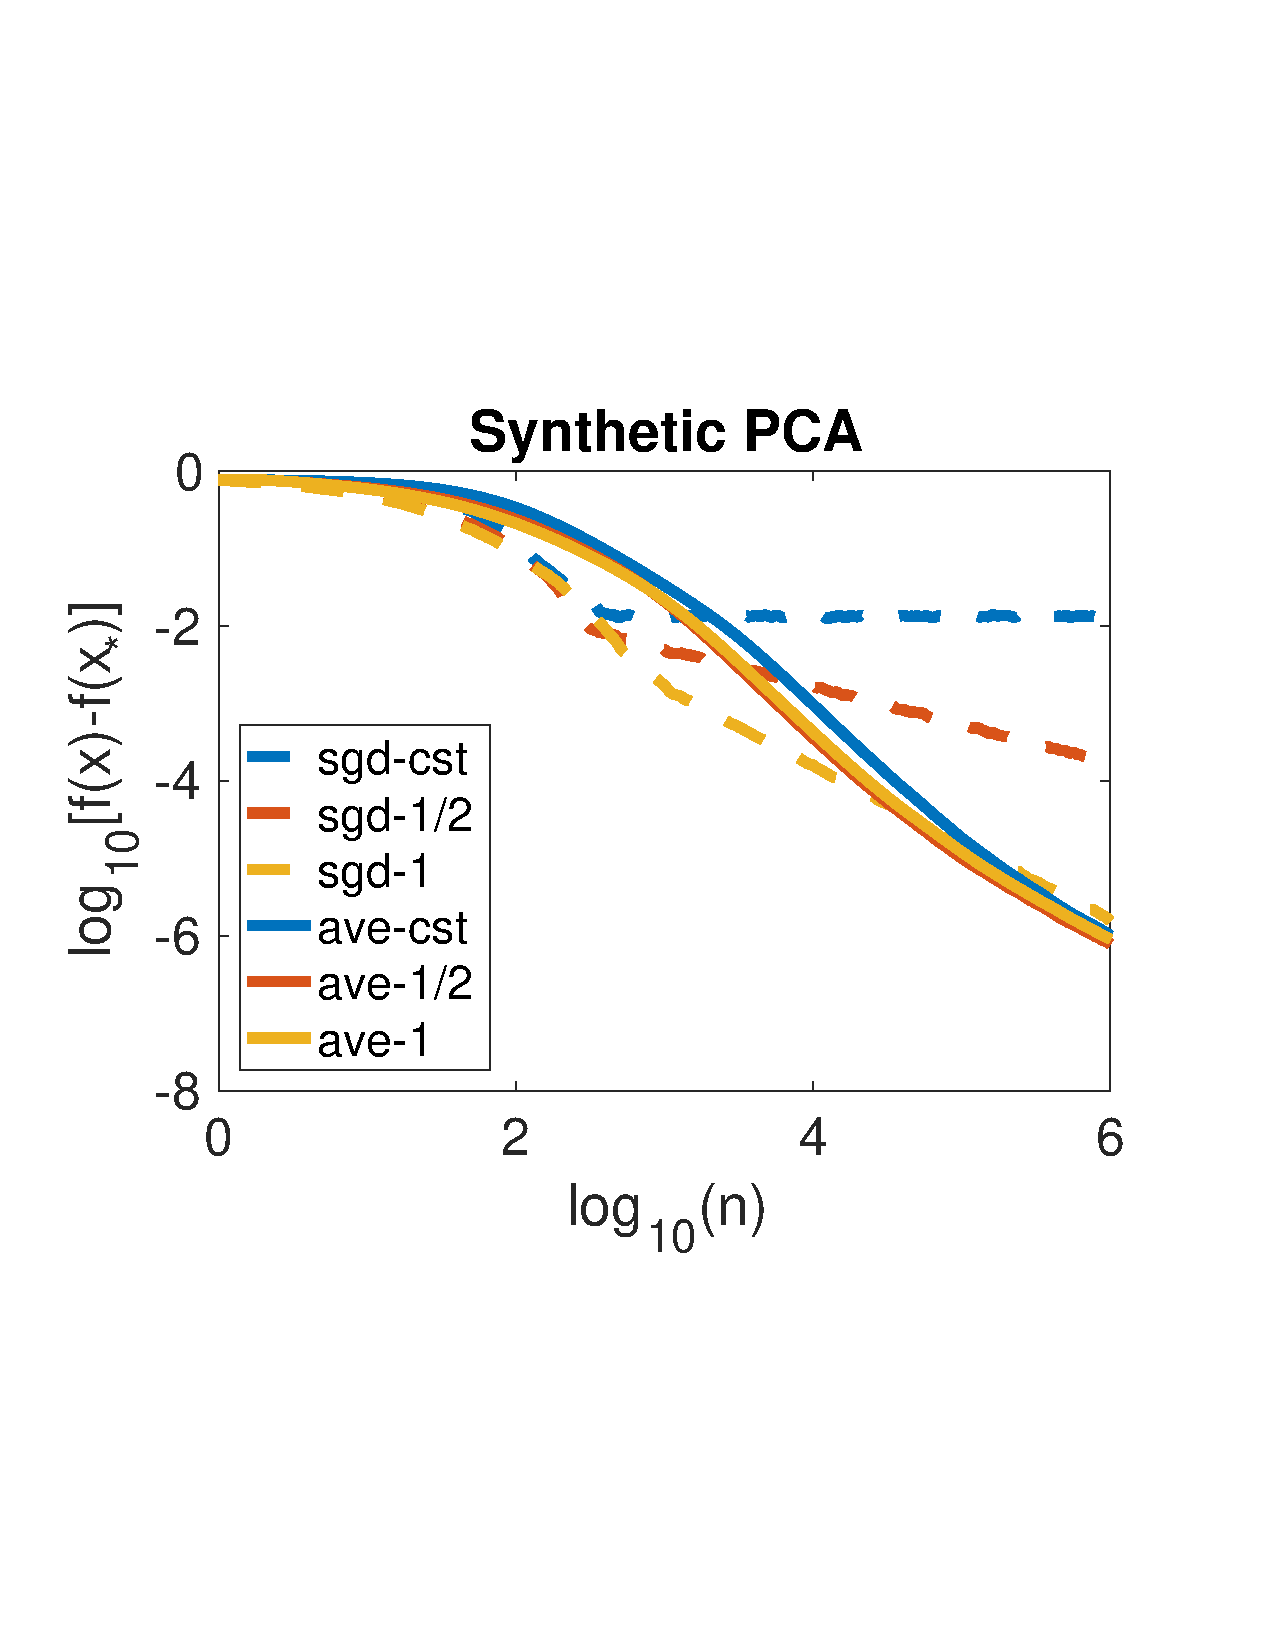
\includegraphics[width=\linewidth]{Figs/gapgrand}
   \end{minipage}
    \hspace*{-10pt}
   \begin{minipage}[c]{.45\linewidth}
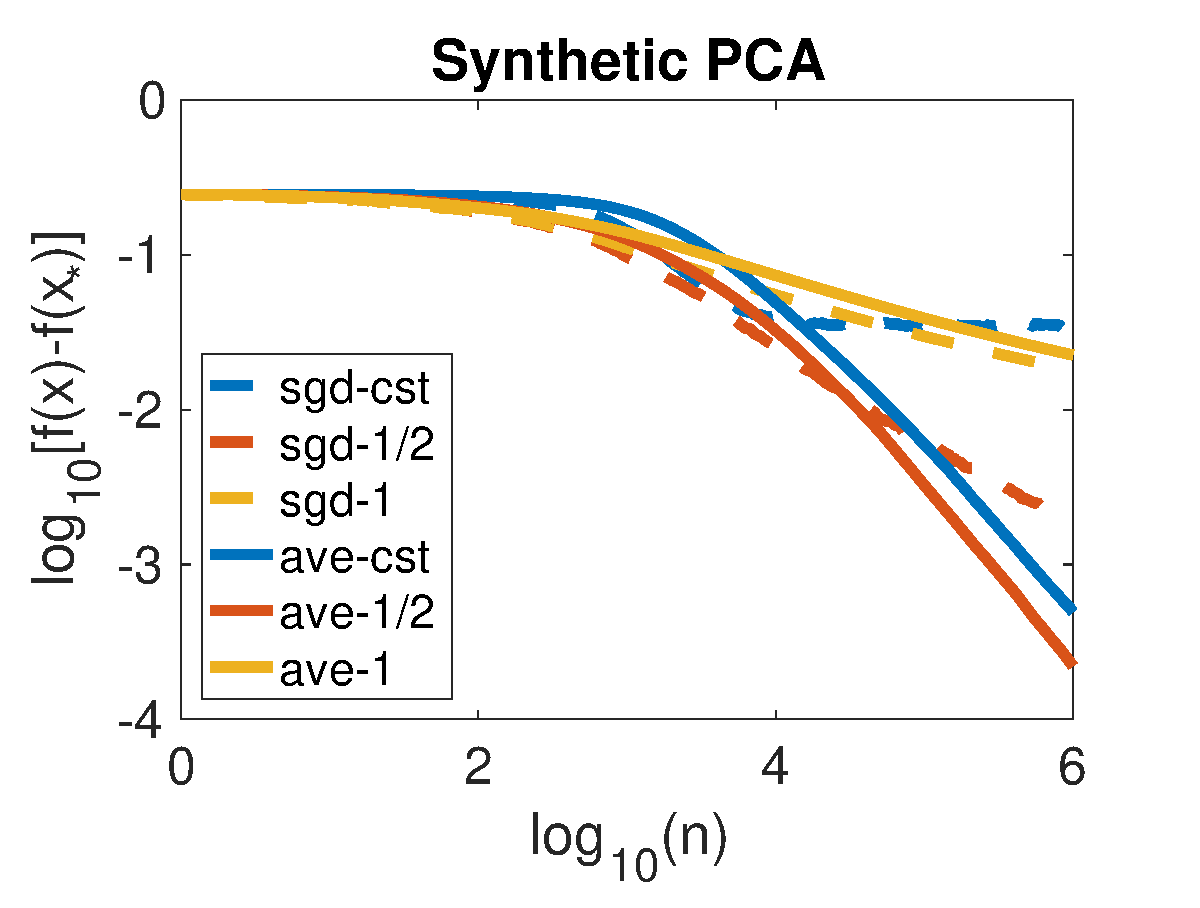
\includegraphics[width=\linewidth]{Figs/gappetit}
   \end{minipage}
   \vspace{-2.25cm}
  \caption{Streaming PCA. Left: Well-conditioned problem. Right: Poorly-conditioned problem.}
     \label{fig:synthetic}
  \vspace{-0.2cm}
\end{figure}
\begin{theorem} \label{thm:oja_main}
  Let Assumption~\ref{assump:manifold} hold for the set $\X = \{ X : \Vert X_\star^\top X\Vert_F^2 \geq k-\eta \}$, for some constant $0 < \eta <\frac{1}{4}$, where $X_\star$ minimizes $f(X)$ over the $k$-Grassmann manifold. Denote, $\tilde{H}_n =  H^{-1/2} H_n H^{-1/2}$, and the 4th-order tensor $C_{ii'jj'} = \E [(v_i^\top \tilde H_n v_j) (v_{i'}^\top \tilde H_n v_{j'})]$. Further assume that $\norm{H_n}_2 \leq 1$ a.s., and that $\lambda_k > \lambda_{k+1}$. Then if $X_n$ and $\tilde{X}_n$ evolve according to \eq{robust_oja}, there exists a positive-definite matrix $C$, such that $\tilde{\Delta}_n = R_{X_{\star}}^{-1}(\tilde{X}_n)$ satisfies:
  \vspace*{-6pt}
  \begin{align}
   \sqrt{n} \tilde{\Delta}_n \overset{D}{\to}  \mathcal{N}(0, C) \ \ \text{ with } \ \     C = \sum_{j'=1}^k\sum_{i'=k+1}^d \sum_{j=1}^k\sum_{i=k+1}^d C_{ii'jj'} \frac{\sqrt{\lambda_i \lambda_j} \cdot \sqrt{\lambda_{i'} \lambda_{j'}}}{(\lambda_{j}-\lambda_{i}) \cdot (\lambda_{j'}-\lambda_{i'})} (v_i e_j^\top) \otimes (v_{i'} e_{j'}^\top). \notag
  \end{align}
\end{theorem}
We  make the following observations:
\begin{itemize}
\vspace*{-6pt}
  \item If the 4th-order tensor satisfies\footnote{For example if $H_n = h_n h_n^\top$ for $h_n \sim \mathcal{N}(0, \Sigma)$ -- so $H_n$ is a rank-one stream of Gaussian random vectors -- this condition is satisfied. See the proof of Theorem \ref{thm:oja_main} for more details.} $C_{ii'jj'} = \kappa \delta_{ii'}\delta_{jj'}$ for constant $\kappa$, the aforementioned covariance structure simplifies to 
$
    C = \kappa \sum_{j=1}^k\sum_{i=k+1}^d\frac{{\lambda_i \lambda_j}}{(\lambda_j-\lambda_i)^2} (v_i e_j^\top) \otimes (v_{i} e_{j}^\top)
    $.
  This asymptotic variance matches the result
  of \citet{reiss2016non}, achieving the same statistical performance as the empirical risk minimizer and matching the lower bound
  of \citet{CaiMaWu13} obtained for the (Gaussian) spiked covariance model. 
  \vspace*{-6pt}
  \item Empirically, even using a constant step size in \eq{robust_oja} appears to yield convergence in a variety of situations; however, we can see a numerical counterexample in \myapp{counter}. We leave it as an open problem to understand the convergence of the iterate-averaged, constant step-size algorithm in the case of Gaussian noise \citep{BouLac85}.
  \vspace*{-6pt}
 \item Assumption~\ref{assump:manifold} could be relaxed using a martingale concentration result showing the iterates $X_n$ are restricted to $\X$ with high probability similar to the work of \citet{shamir16b} and \citet{AllenLi2017-streampca}.
 \vspace*{-4pt}
\end{itemize}
Note that we could also derive an analogous result to Theorem \ref{thm:oja_main} for the (averaged) Riemannian SGD algorithm in \eq{grad_desc} and \eq{ave_grad_desc}. However, we prefer to present the algorithm in \eq{robust_oja} since it is simpler and directly averages the (commonly used) randomized power method.
